% Unofficial University of Cambridge Poster Template
% https://github.com/andiac/gemini-cam
% a fork of https://github.com/anishathalye/gemini
% also refer to https://github.com/k4rtik/uchicago-poster

\documentclass[final]{beamer}

% ====================
% Packages
% ====================

\usepackage[T1]{fontenc}
\usepackage[orientation=portrait,size=a4,scale=1.2]{beamerposter}
\usetheme{gemini}
\usecolortheme{nott}
\usepackage{graphicx}
\usepackage{booktabs}
\usepackage{tikz}
\usepackage{pgfplots}
\pgfplotsset{compat=1.14}
\usepackage{anyfontsize}
\usepackage{subcaption}
\usepackage{array}


% ====================
% Lengths
% ====================

% If you have N columns, choose \sepwidth and \colwidth such that
% (N+1)*\sepwidth + N*\colwidth = \paperwidth
\newlength{\sepwidth}
\newlength{\colwidth}
\setlength{\sepwidth}{0.02\paperwidth}
\setlength{\colwidth}{0.47\paperwidth}

\newcommand{\separatorcolumn}{\begin{column}{\sepwidth}\end{column}}

% ====================
% Title
% ====================

\title{A Camera That Sees Behind}

% \author{Agajan Torayev \inst{1} \and Ben Bitdiddle \inst{2} \and Lem E. Tweakit \inst{2}}
\author{
  Yan Lin (lyan@cs.aau.dk)
}

% \institute[shortinst]{
% \inst{1} Department of Computer Science, Aalborg University
% }

% ====================
% Footer (optional)
% ====================

% Footer content removed to maximize space for poster content


% ====================
% Logo (optional)
% ====================

% use this to include logos on the left and/or right side of the header:
\logoleft{\includegraphics[height=1.5cm]{figures/aau.png}}
\logoright{\includegraphics[height=1.5cm]{figures/daisy.png}}

% ====================
% Body
% ====================

\begin{document}


\begin{frame}[c]

% Full-width Project Goal section with largest font
\begin{alertblock}{Project Goal}
{\large
Develop a \textbf{computationally lightweight model} that can be deployed onto embedded devices to \textbf{remove humans from images or video feeds}, revealing the background scene beneath.
The system can serve as a prototype GDPR-compliant surveillance system.
}

\begin{figure}
  \centering
	\includegraphics[width=0.98\linewidth]{figures/system-flow.pdf}
	\label{fig:workflow}
\end{figure}

\end{alertblock}



\begin{columns}[t]
\separatorcolumn

\begin{column}{\colwidth}


\begin{block}{Background \& Motivation}

\begin{figure}
    \centering
    \begin{subfigure}[b]{0.32\textwidth}
        \centering
        \includegraphics[width=\textwidth]{figures/warehouse-faceblur.png}
        \caption{Face blur: Identifiable by body shape or clothing}
        \label{fig:faceblur}
    \end{subfigure}
    \hfill
    \begin{subfigure}[b]{0.32\textwidth}
        \centering
        \includegraphics[width=\textwidth]{figures/warehouse-fullblur.png}
        \caption{Full body blur: Identifiable by posture}
        \label{fig:fullblur}
    \end{subfigure}
    \hfill
    \begin{subfigure}[b]{0.32\textwidth}
        \centering
        \includegraphics[width=\textwidth]{figures/warehouse-inpaint.png}
        \caption{Removed with inpainting: Not identifiable}
        \label{fig:inpaint}
    \end{subfigure}
    \vspace{-.3cm}
\end{figure}

{\large
\begin{enumerate}
\item There are demands for \textit{GDPR-compliant surveillance systems} that do not store personally identifiable information; for example, those deployed in warehouses to keep track of inventory but should avoid storing footage of workers moving inside them
\item GDPR's definition of personally identifiable information is broad enough to include footage from which ``\textit{your mother is able to identify you}''; one of the safest approaches is to remove humans captured in the footage as if they were not there
\end{enumerate}
}

\end{block}



\begin{block}{System Deployment Options}

{\large
\textbf{Embedded devices} for capturing footage and running the developed method locally will be provided. Options include:
}
 

\begin{figure}
    \centering
    \begin{subfigure}[b]{0.47\textwidth}
        \centering
        \includegraphics[width=\textwidth]{figures/jetson.png}
        \caption{NVIDIA Jetson development kit}
        \label{fig:jetson}
    \end{subfigure}
    \hfill
    \begin{subfigure}[b]{0.47\textwidth}
        \centering
        \includegraphics[width=\textwidth]{figures/rpi.jpg}
        \caption{Raspberry Pi 5}
        \label{fig:rpi}
    \end{subfigure}
    \vspace{-.3cm}
\end{figure}

{\large
\begin{enumerate}
\item \textit{Nvidia Jetson}: a powerful embedded device with 4-core CPU, 8GB RAM, and Nvidia GPU; the GPU can be used to accelerate the computation of ML models (especially neural network models)
\item \textit{Raspberry Pi}: a power-efficient embedded device with 4-core CPU and 4GB RAM; very good official and community support for development
\end{enumerate}
Both options include a compatible camera for capturing footage.
}


\end{block}


\end{column}


\separatorcolumn

\begin{column}{\colwidth}

\begin{block}{Requirements \& Challenges}

{\large
A method needs to be developed that can \textbf{identify humans from footage} (images or videos) and \textbf{inpaint the area with a realistic background}; potential directions include:
\begin{enumerate}
\item \textit{Two-stage approach}: first, detect the area occupied by humans as a mask; second, inpaint the masked area with an ML-generated background
\item \textit{One-stage approach}: an ML model that accepts footage with humans and outputs manipulated footage without humans in an end-to-end manner
\end{enumerate}
}

\begin{figure}
  \centering
	\includegraphics[width=\textwidth]{figures/approaches.pdf}
	\label{fig:approaches}
\end{figure}

{\large
The method also needs to be \textbf{lightweight enough to be deployed onto embedded devices}, so that the captured footage with humans can be processed in near real-time (i.e., unprocessed footage is not stored for GDPR-compliance); potential directions include:
\begin{enumerate}
\item \textit{Lightweight neural network architectures}: for example, U-Net that can achieve good performance with fewer parameters
\item \textit{Efficient computing techniques}: for example, low-precision floating-point inference that can accelerate ML model computation without sacrificing performance
\end{enumerate}
}

\begin{figure}
    \centering
    \begin{subfigure}[b]{0.5\textwidth}
        \centering
        \includegraphics[width=\textwidth]{figures/unet.png}
        \caption{U-Net structure}
        \label{fig:unet}
    \end{subfigure}
    \hfill
    \begin{subfigure}[b]{0.45\textwidth}
        \centering
        \includegraphics[width=\textwidth]{figures/tensorrt.jpg}
        \caption{Nvidia's inference acceleration framework}
        \label{fig:tensorrt}
    \end{subfigure}
    \vspace{-.3cm}
\end{figure}


\end{block}


\rule{\textwidth}{0.4pt}

{\small
\begin{enumerate}
\item Mask extraction models: https://www.geeksforgeeks.org/python/python-foreground-extraction-in-an-image-using-grabcut-algorithm/
\item Inpainting models: https://huggingface.co/docs/diffusers/en/using-diffusers/inpaint
\end{enumerate}
}


\end{column}
\separatorcolumn

\end{columns}

\end{frame}

\end{document}
